\documentclass{article}
\usepackage[utf8]{inputenc}
\usepackage{array}
\usepackage{amsmath}
\usepackage{graphicx,float}
\usepackage{subfigure}
\usepackage{csvsimple}
\begin{document}
\begin{table}[h!]
\begin{center}
\caption{Student Data}
\label{tab:Table1}
\vspace{5mm}
\begin{tabular}{|c|c|c|c|c|}
\textbf{Name} & \textbf{Division} & \textbf{MIS} & \textbf{Year of Birth} & \textbf{Branch}\\
\hline
Abhinav & 8 & 112103004 & 2002 & Computer\\
Akshay & 1 & 112105002 & 2002 & Instrumentation\\
Kevin & 9 & 112107035 & 2003 & Electrical\\
Rakesh & 6 & 112106071 & 2003 & Electronics\\
Aakash & 3 & 112102009 & 2004 & Civil\\
\end{tabular}
\end{center}
\end{table}
\vspace{30mm}
\begin{table}[h!]
\begin{center}
\caption{Movie preferences}
\label{tab:Table2}
\vspace{5mm}
\begin{tabular}{|l|c|c|c|}
\hline
\textbf{Name} & \textbf{Genre} & \textbf{Fav. Actor/Actress} & \textbf{Fav. Film}\\
\hline
Snehasish & Suspense,thriller & Benedict Cumberbatch & Manchester by the sea,Whiplash\\
\hline
Sahil & Rom-coms & Shahrukh Khan & DevDas\\
\hline
Indraneel & Sci-Fi & Tom Cruise & Arrival\\
\hline
Bhavika & Action & Keanu Reeves & John Wick\\
\hline




\end{tabular}
\end{center}
\end{table}
\vspace{50mm}
\section*{Section : Matrix Applications}
\begin{enumerate}
 \item Find the rank and bases for the row and column spaces of following matrices:
\[
A =
\begin{pmatrix}
1 & 3 & 4 \\
2 & -6 & 9 \\
2 & -6 & 9 \\
-1 & 3 & -4 \\

\end{pmatrix}
\]
 \item Show that the three points $(x_1, y_1),(x_2, y_2),(x_3, y_3)$ in a plane are collinear if and only if the following matrix has rank less than 3.
\begin{center}
\[
M =
\begin{bmatrix}
x_1 & y_1 & 1 \\
x_2 & y_2 & 1 \\
x_3 & y_3 & 1 \\

\end{bmatrix}
\]
\end{center}
\item Determine whether B is in the column space of A, and if so, express B as a linear combination of the column vectors of A: 
\begin{equation*}
A =
\begin{pmatrix}
1 & 1 & 2 \\
1 & 0 & 1 \\
2 & 1 & 3 \\
\end{pmatrix}
,\,
B =
\begin{pmatrix}
-1 \\
0 \\
2 \\
\end{pmatrix}
\end{equation*}

\end{enumerate}
\pagebreak
\begin{center}
\section*{Section : Figure Insertion}
\end{center}

\begin{figure}[!h]
\begin{center}
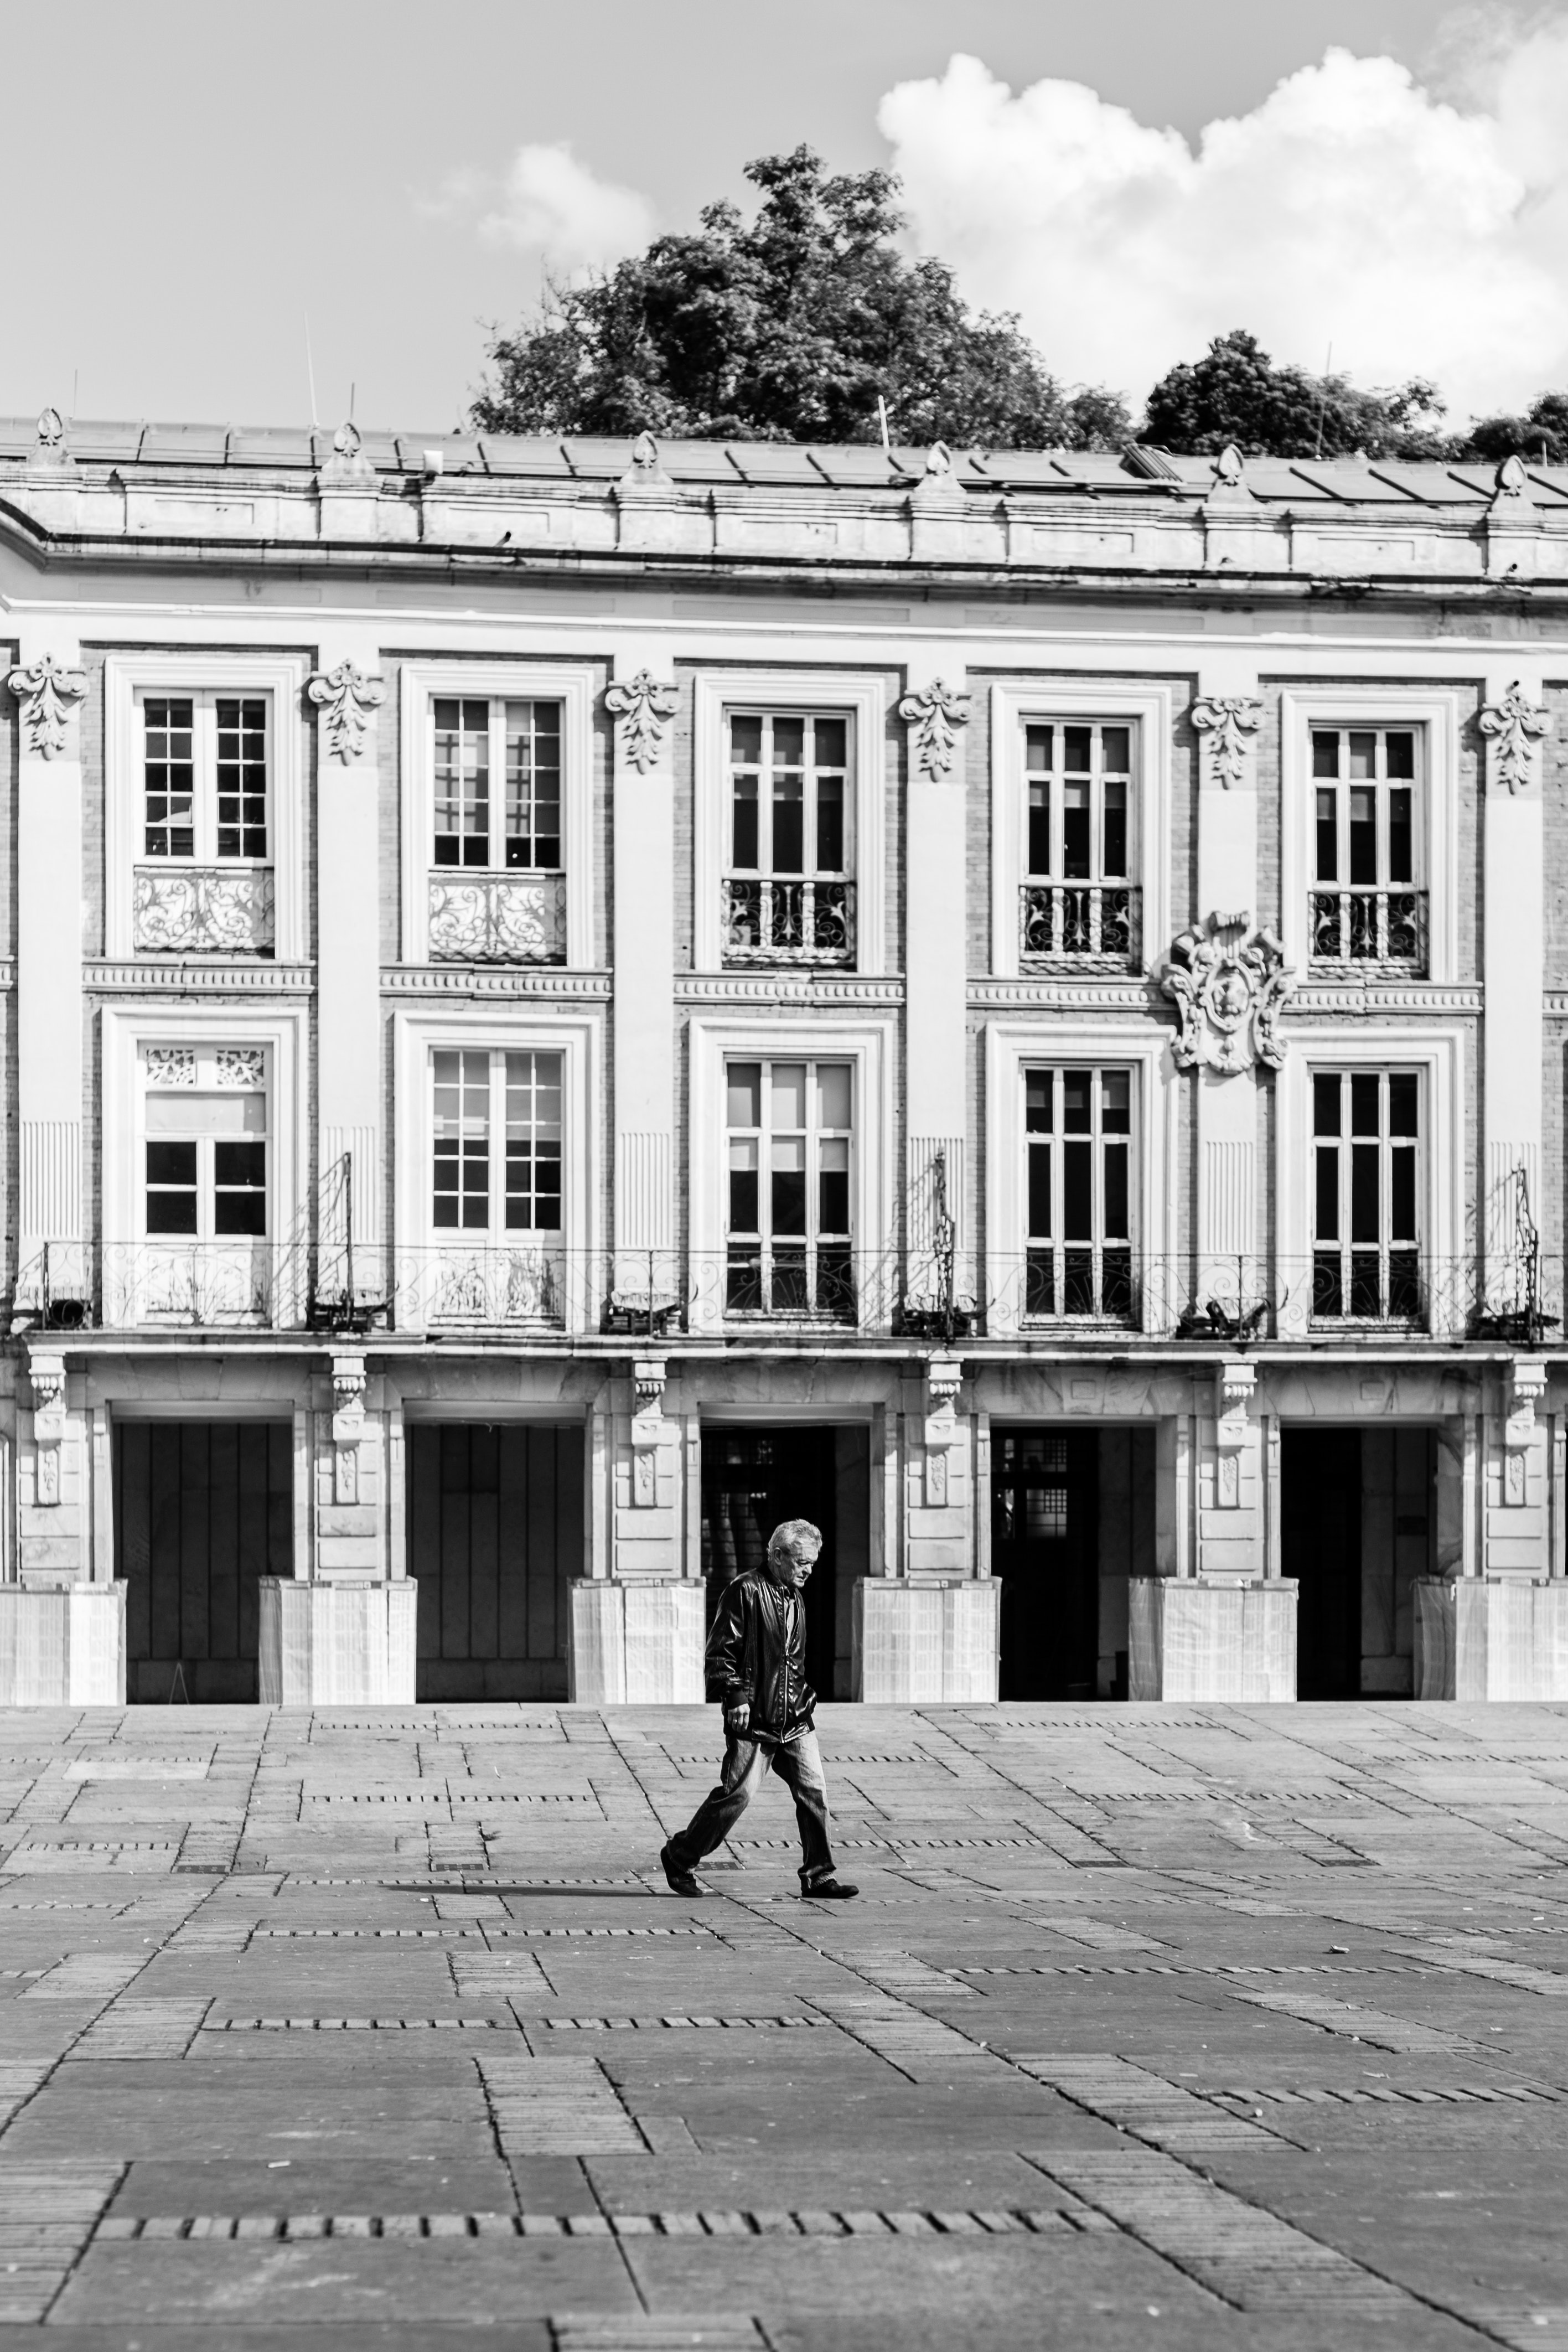
\includegraphics[width=0.65\textwidth]{latex.jpg}
\end{center}
\caption{Leisure Strolling}
\end{figure}
\pagebreak
\begin{figure}[!h]
\begin{center}
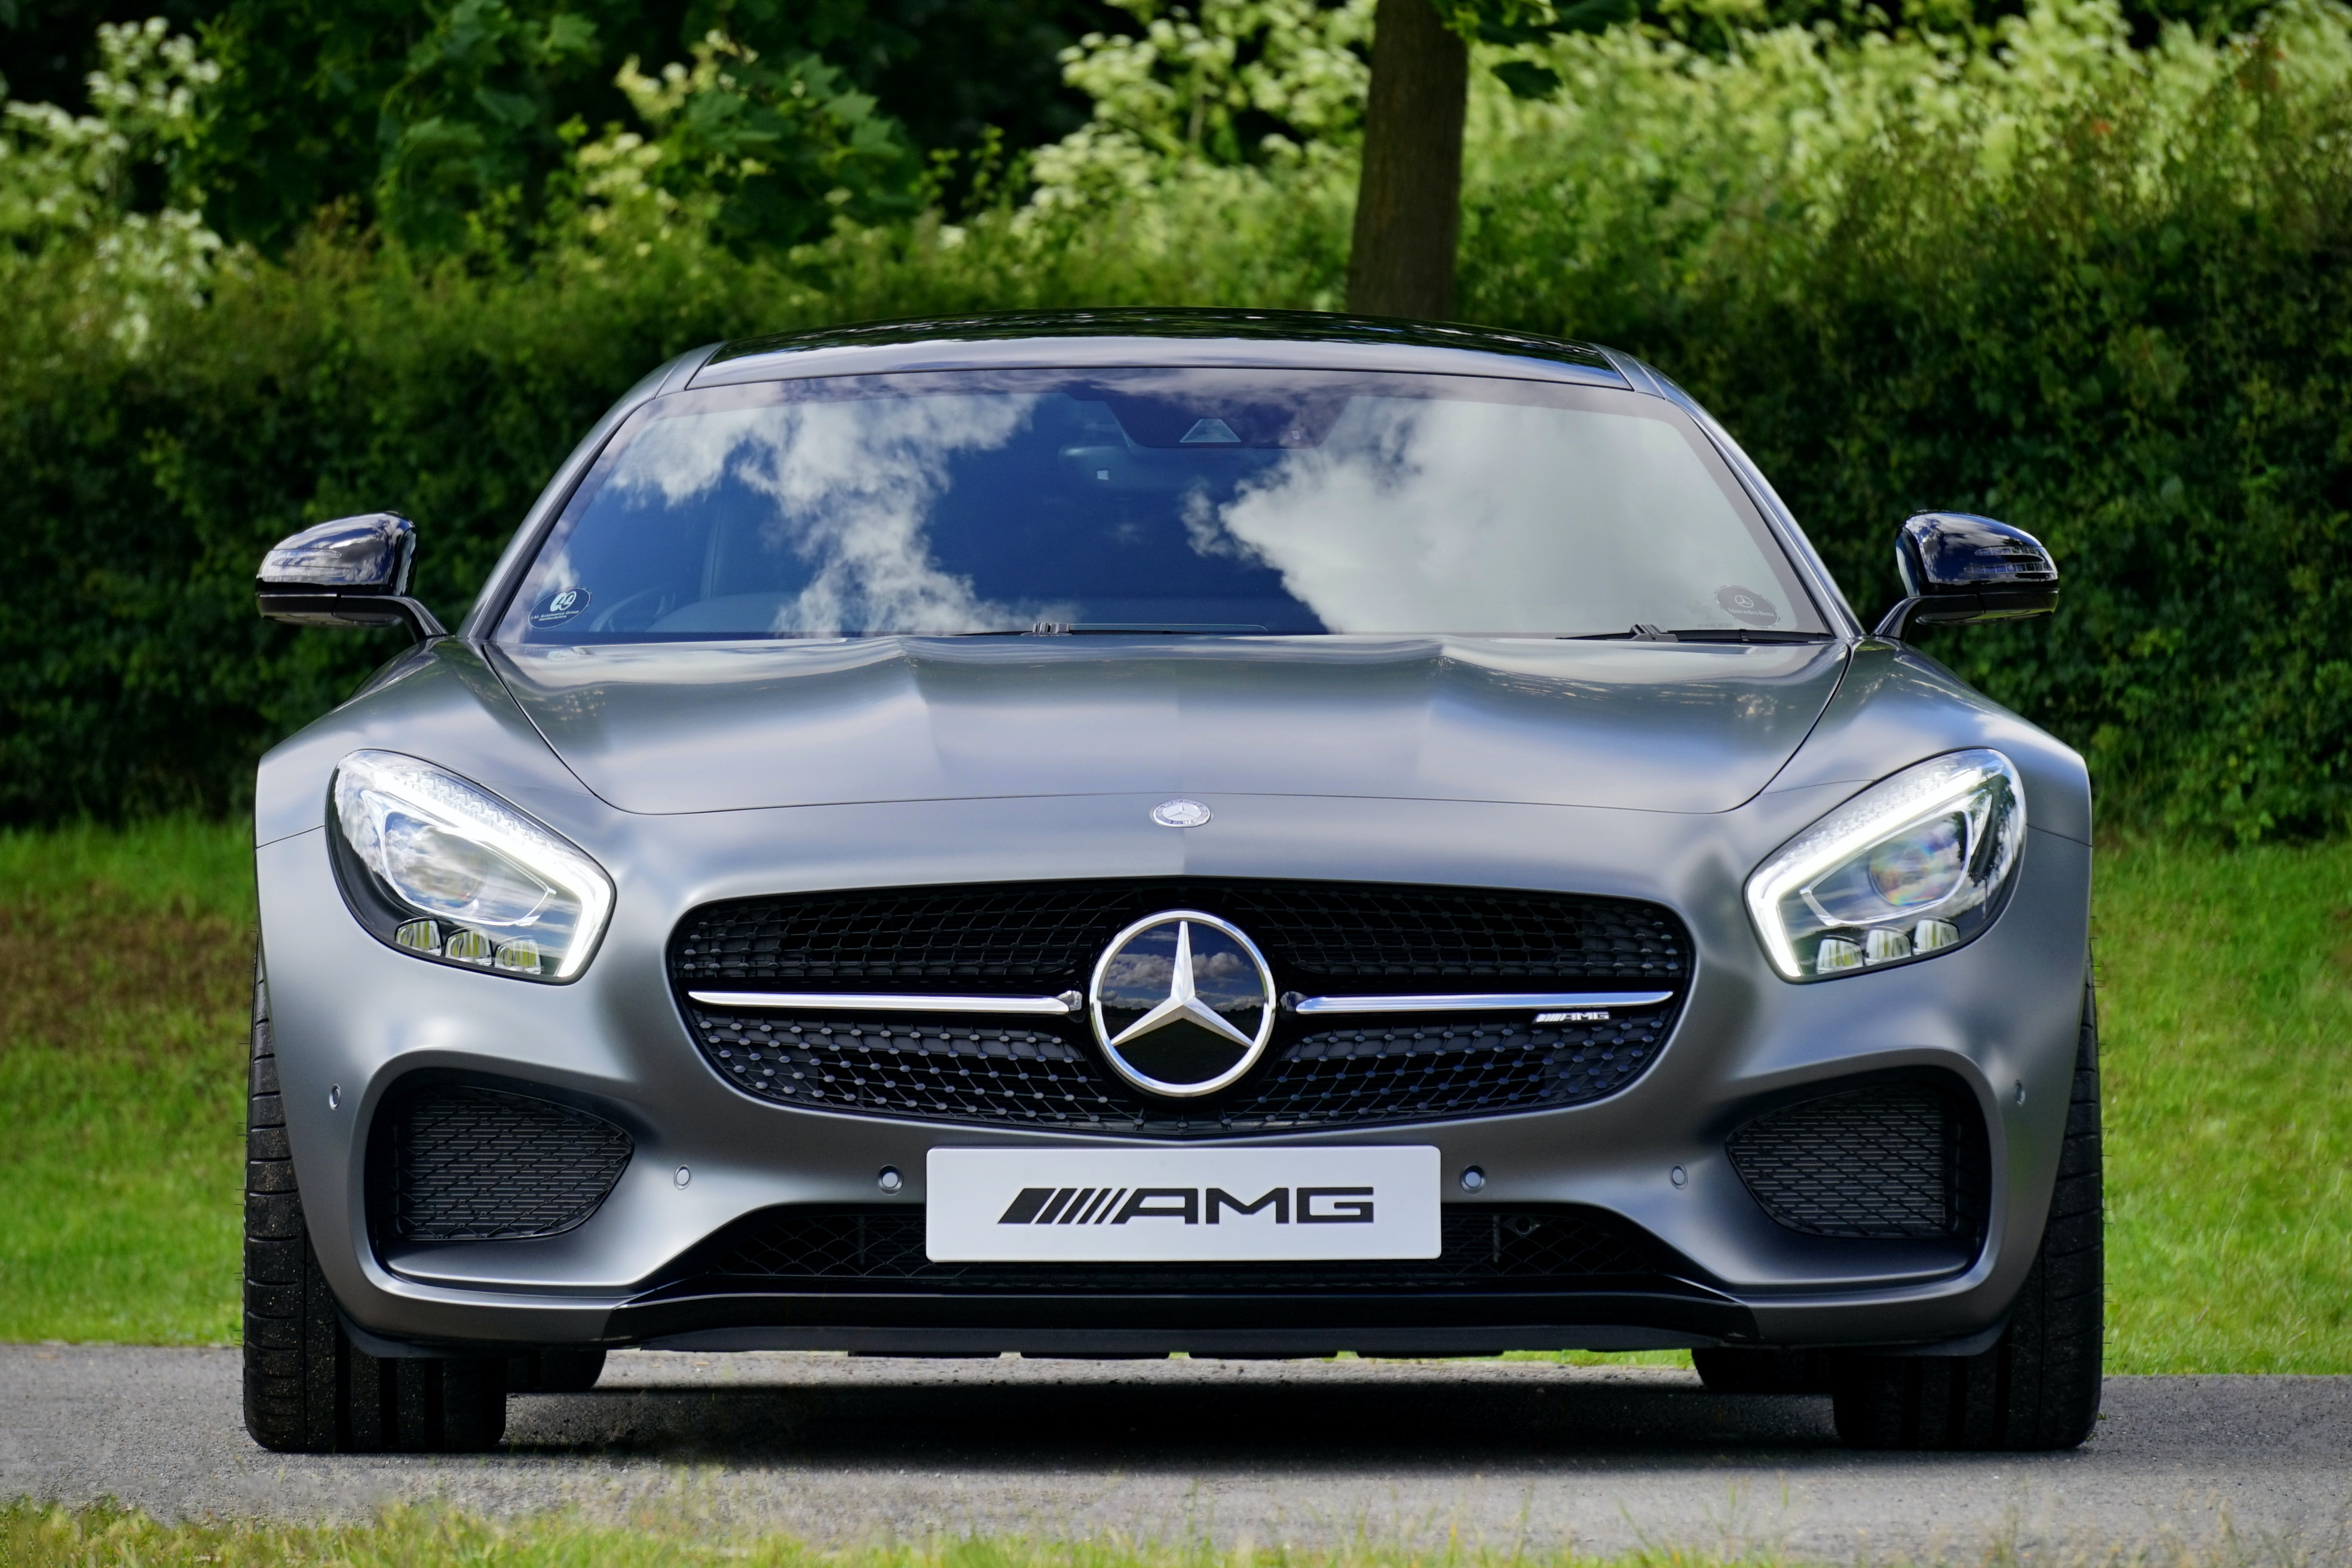
\includegraphics[width=1.0\textwidth]{car.jpg}
\end{center}
\caption{AMG}
\end{figure}
\pagebreak
\begin{table}[H]
\csvautotabular{data.csv}
\end{table}


\end{document}